\documentclass[../main.tex]{subfiles}

\begin{document}
%%%%%%%%%%%%%%%%%%%%%%%%%%%%%
%                           %
% GRENZWERTE UND STETIGKEIT %
%                           %
%%%%%%%%%%%%%%%%%%%%%%%%%%%%%

\chapter{Grenzwerte und Stetigkeit}
\section{Grenzwert}
$\lim\limits_{x\to a}f(x)=L$ oder $f(x)\to L$, falls $x\to a$.

\subsection{Linksseitiger Grenzwert}
$\lim\limits_{x\to a^-}f(x)$

\subsection{Rechtsseitiger Grenzwert}
$\lim\limits_{x\to a^+}f(x)$

\subsection{Zweiseitiger Grenzwert}
Der zweiseitige Grenzwert existiert genau dann, wenn links- und rechtsseitiger Grenzwert exisitieren und diese gleich sind: \\ [7pt]
$\lim\limits_{x\to a}f(x)=L$ genau dann, wenn $\lim\limits_{x\to a^-}f(x)=L=\lim\limits_{x\to a^+}f(x)$

\subsection{Uneigentliche Grenzwerte}
Grenzwert wächst bis über alle Grenzen wenn man $x$ gegen $a$ gehen lässt: \\ [7pt]
$\lim\limits_{x\to a}f(x)=\infty$

\subsection{Grundlegende Grenzwerte Theorem}
\begin{math}
    \lim\limits_{x\to a} k = k \\ [7pt]
    \lim\limits_{x\to a} x = a \\ [7pt]
    \lim\limits_{x\to 0^-} \frac{1}{x} = -\infty \\ [7pt]
    \lim\limits_{x\to 0^+} \frac{1}{x} = \infty
\end{math}

\subsection{Rechnen mit Grenzwerten}
\subsubsection{Theorem Summe}
Falls $a \in \mathbb{R} \cup \{ -\infty, +\infty\}, \mu,\nu \in \mathbb{R}$ und \\ [7pt]
$\lim\limits_{x\to a} f(x) = L_1$ und $\lim\limits_{x\to a} g(x) = L_2$ dann gilt: \\ [14pt]

\textbf{Der GW einer Summe/Differenz ist gleich der Summe/Differenz der GWs; Konstanten kommen vor den GW:} \\ [7pt]
$\lim\limits_{x\to a}[\mu f(x) \pm \nu g(x)] = \mu \lim\limits_{x\to a} f(x) \pm \nu \lim\limits_{x\to a} g(x) = \mu L_1 \pm \nu L_2$

\subsubsection{Theorem Produkt}
\textbf{Der GW eines Produkts ist gleich dem Produkt der GWs:} \\ [7pt]
$\lim\limits_{x\to a}[f(x)g(x)] = \lim\limits_{x\to a} f(x) \times \lim\limits_{x\to a} g(x) = L_1L_2$

\subsubsection{Theorem Quotient}
Ist $L_2 \neq 0$ und g in einer Umgebung von $a$ verschieden von $0$, dann ist der \textbf{GW des Quotienten gleich dem Quotienten der GWs:} \\ [7pt]
$\lim\limits_{x\to a}[\frac{f(x)}{g(x)}] = \frac{\lim\limits_{x\to a}f(x)}{\lim\limits_{x\to a}g(x)} = \frac{L_1}{L_2}$ \\ [7pt]
Siehe \hyperref[sec:GW_Quotient]{\ref{sec:GW_Quotient} \nameref{sec:GW_Quotient}} für Beispiel.


\subsubsection{Folgerungen Exponent}
\begin{tabularx}{0.8\textwidth} { 
    >{\centering\arraybackslash}X 
    >{\centering\arraybackslash}X  }
    \begin{math}
        \lim\limits_{x\to a} x^n = (\lim\limits_{x\to a} x)^n = a^n
    \end{math}
    &
    \begin{math}
        \lim\limits_{x\to a} [f(x)]^n = (\lim\limits_{x\to a} f(x))^n
    \end{math}
\end{tabularx}

\subsubsection{Folgerungen Polynom}
Für ein Polynom $p(x) = c_0 + c_1x + ... + c_nx^n = \sum\limits_{k=0}^n c_kx^k$ gilt: \\[7pt]
$\lim\limits_{x\to a} p(x) = c_0 + c_1x + ... + c_nx^n = p(a)$ \\ [7pt]
Siehe \hyperref[sec:GW_Polynom]{\ref{sec:GW_Polynom} \nameref{sec:GW_Polynom}} für Beispiel.

\subsubsection{Folgerungen Quotient}
Für eine rationale Funktion $r(x) = \frac{p(x)}{q(x)}$ (dabei sind $p(x)$ und $q(x)$ Polynome) und eine $a \in \mathbb{R}$ gilt: \\
(a) Falls $q(a) \neq 0$, dann ist $\lim\limits_{x\to a} r(x) = r(a)$ \\
(b) Falls $q(a) = 0$ und $p(a) \neq 0$, dann existiert $\lim\limits_{x\to a} r(x)$ nicht. \\
(c) Falls $q(a) = 0$ und $p(a) = 0$, dann kann der GW existieren, muss aber nicht!
Siehe \hyperref[sec:GW_Quotient]{\ref{sec:GW_Quotient} \nameref{sec:GW_Quotient}} für Beispiel.

\subsection{Squeezing-Theorem}
Gilt für drei Funktionen f, g und h in einer Umgebung von c (evt. mit Ausnahme von c) \\ [7pt]
$g(x) \le f(x) \le h(x)$ und $\lim\limits_{x\to c} g(x) = \lim\limits_{x\to c} h(x) = L$ \\ [7pt]
dann gilt auch $\lim\limits_{x\to c} f(x) = L$

\section{Stetigkeit}
Salopp: Eine Funktion f heisst stetig, wenn man deren Graphen zeichnen kann, ohne den Stift absetzen zu müssen. \\ [7pt]
Genauer ist eine Funktion f stetig in a, falls:
\begin{itemize}
    \item Die Funktion f dort existiert, d.h. falls $f(a)$ definiert ist.
    \item Links- und rechtsseitiger Grenzwert existieren und gleich sind \\ [7pt]
    $\lim\limits_{x\to a^-} f(x) = \lim\limits_{x\to a^+} f(x) = \lim\limits_{x\to a} f(x)$ 
    \item Die genannten Grenzwerte mit dem Funktionswert übereinstimmen.
\end{itemize}
Zusammengefasst: f ist stetig in a, falls \\ [7pt]
$\lim\limits_{x\to a} f(x) = f(a)$ \\ [7pt]
Eine Funktion heisst stetig, falls sie überall, d.h. $\forall x \in D(f)$ stetig ist.

\subsection{Grenzwert einer Funktion von x - Theorem}
Sei $a \in \mathbb{R} \cup \{ -\infty, +\infty\}$. Gilt dann $\lim\limits_{x\to c} g(x)=L$ und ist $f$ im Punkt L stetig, dann gilt: \\ [7pt]
$\lim\limits_{x\to c} f(g(x)) = f(\lim\limits_{x\to c} g(x))$ \\ [7pt]
Insbesondere gilt zB \\ [7pt]
$\lim\limits_{x\to c} |g(x)| = |(\lim\limits_{x\to c} g(x)|$ \\ [7pt]
falls $\lim\limits_{x\to c} g(x)$ existiert!

\subsection{Rechenregeln}
\begin{itemize}
    \item Summe und Differenz stetiger Funktionen sind stetig.
    \item Der Quotient zweier stetiger Funktionen ist dort stetig, wo der Nenner nicht verschwindet.
    \item Polynome $p(x) = \sum\limits_{k=0}^n a_kx^k$ sind stetig.
    \item Rationale Funktionen $r(x) = \frac{p(x)}{q(x)}$ sind dort stetig, wo das Nennerpolynom $q(x)$ nicht verschwindet.
    \item Sinus- $(\sin x)$ und Kosinusfunktion $(\cos x)$ sind stetig.
    \item Der Tangens $(\tan x = \frac{\sin x}{\cos x})$ ist stetig, falls $\cos x \neq 0$, dh falls $x \neq \frac{\pi}{2} + k \pi, k \in \mathbb{Z}$.
    \item Exponential- und Logarithmusfunktionen sind in ihrem Definitionsbereichen stetig.
    \item Zusammensetzung stetiger Funktionen ist stetig.
    \item Eine zusammegesetzte Funktion kann dort unstetig sein, wo eine der verwendeten Funktionen nicht stetig ist.
\end{itemize}

\subsection{Eigenschaften stetiger Funktionen}
\subsubsection{Theorem Zwischenwertsatz}
Ist $f$ im Interval $[a,b]$ stetig, dann nimmt $f$ jeden Wert zwischen $f(a)$ und $f(b)$ (inklusive) mindestens einmal an.
\subsubsection{Corollary - Nullstellensatz von Bolzano}
Ist $f$ auf $[a,b]$ stetig und gilt $f(a)f(b) < 0$, dann besitzt $f$ in $[a,b]$ wenigstens eine Nullstelle, dh. $\exists x \in [a,b]$ mit $f(x)=0$ \\
In anderen Worten: Wenn eine Funktion im Bereich $[a,b]$ stetig ist und es vom Intervall $a$ zu $b$ einen Vorzeichenwechsel gibt, dann gibt es mindestens eine Nullstelle.

\subsection{Regula Falsi}
Basierend auf dem Nullstellensatz von Bolzano.

\begin{minipage}{0.5\textwidth}
        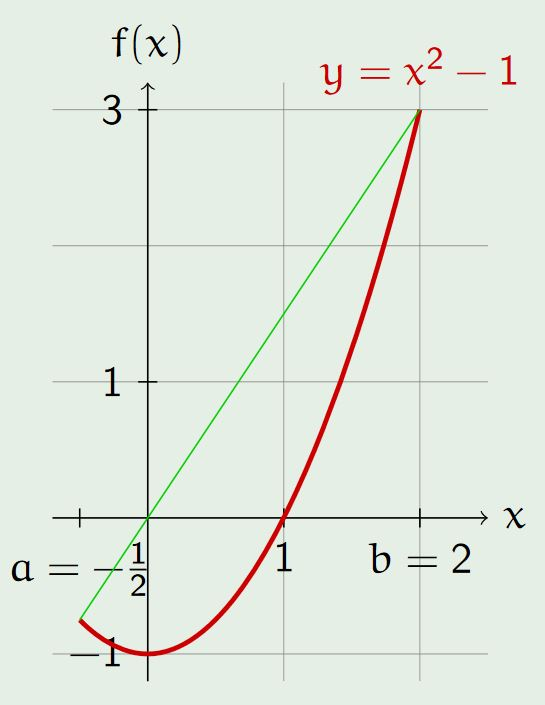
\includegraphics[width=50mm,scale=0.5]{regula_falsi}
\end{minipage} \hfill
\begin{minipage}{0.45\textwidth}
    Der Schnittpunkt der Sekante (grün) durch $(a, f(a))$ und $(b, f(b))$ mit der x-Achse ergibt eine erste Näherung für die Nullstelle (NS) von f: \\ [7pt]
    $x = a-f(a) \frac{b-a}{f(b)-f(a)} = \frac{af(b)-bf(a)}{f(b)-f(a)}$  \\ [7pt]
    Gilt dann $f(x)f(a)<0$, dann liegt die NS im Intervall $[a,x]$, sonst in $[b,x]$. \\
    Wiederhole die Prozedur mit dem Intervall welches die NS enthält!
\end{minipage}


\section{Beispiele}
\subsection{Geschickt erweitern}
\begin{math}
    \lim\limits_{x\to 1} \frac{x-1}{\sqrt{x}-1} =
    \lim\limits_{x\to 1} \frac{x-1}{\sqrt{x}-1} \times \frac{\sqrt{x}+1}{\sqrt{x}+1} =
    \lim\limits_{x\to 1} \frac{(x-1)(\sqrt{x}+1)}{x-1} = \\ [7pt]
    \lim\limits_{x\to 1} (\sqrt{x}+1) =
    \lim\limits_{x\to 1} \sqrt{x} + \lim\limits_{x\to 1} 1 =
    1 + 1 = 2
\end{math}

\subsection{GW Polynom}
\label{sec:GW_Polynom}
\begin{math}
    \lim\limits_{x\to 1} (x^7 - 2x^5 + 1)^{35} = (1^7 - 2 \times 1^5 +  1)^{35} = 0
\end{math}

\subsection{GW Quotient}
\label{sec:GW_Quotient}
\begin{math}
    \lim\limits_{x\to 2} \frac{5x^3 + 4}{x -3} = \frac{\lim\limits_{x\to 2}5x^3 + 4}{\lim\limits_{x\to 2}x -3}
\end{math}
und wegen der Regel für Polynome: \\ [7pt]
\begin{math}
    \lim\limits_{x\to 2} \frac{5x^3 + 4}{x -3} = \frac{5 \times 2^3 + 4}{2 -3} = -44
\end{math}


\end{document}